\documentclass{article}
\usepackage{graphicx}
\begin{document}
\title{Masters Thesis}
\author{Alvaro Prieto\\
BS/MS Electrical Engineering\\
\texttt{axp8664@rit.edu}}
\maketitle

\pagebreak

\tableofcontents

\pagebreak

\begin{abstract}
...
\end{abstract}

\section{Summary of Contributions}
\begin{itemize}
\item BSN Software Libraries
\item wireless ECG platform
\item New routing algorithm
\end{itemize}
% Include literature survey from other file
\section{Literature Survey}\label{section:litsurvey}
\subsection{Time Synchronization}
Time synchronization has been the subject of research for many years.

There are robust and time-tested synchronization methods, such as the Network Time Protocol (NTP)~\cite{synchronization:NTP}, which are currently in use around the world. Unfortunately these methods were designed for wired systems, and do not perform well once power consumption, latency, and other wireless effects taken into account. 

One of the first synchronization protocols designed specifically for wireless networks is Reference Broadcast Synchronization (RBS)~\cite{synchronization:RBS}. The main idea behind RBS is to synchronize all wireless sensor nodes to each other. This creates a local time, within the network of nodes, where all clocks are synchronized. For many applications, sensor nodes do not need to know the actual time, as long as they are synchronized to one another. \cite{synchronization:RBS} lists an example application that measures the time-of-flight of sound. If needed, RBS can be extended to use an external global time source to provide a relate the local and global times.

There are several sources of nondeterminism in a wireless network. ~\cite{synchronization:RBS} and ~\cite{synchronization:FTSP} decompose the sources of nondeterminism into several components. These components account for the delays due to the sending and receiving of a message in a wireless network. These components(from ~\cite{synchronization:RBS}) are: 
\begin{itemize}
\item \emph{Send Time} -- Time the sender takes to construct a message. Includes delays incurred by the operating system and time required to transfer the message from the host to the network interface.
\item \emph{Access Time} -- Time spent waiting for access to transmit channel.
\item \emph{Propagation Time} -- Time taken by the message to physically travel from sender to receiver.
\item \emph{Receive Time} -- Time spent processing a message and notifying the host of its arrival.
\end{itemize}

As suggested by its name, RBS uses broadcast messages to synchronize wireless nodes to one another. RBS does not synchronize a set of wireless nodes to a reference clock. Because of this property, RBS effectively eliminates the \emph{Send Time} and \emph{Access Time} as sources of error. The \emph{Access Time}, while unknown, is the same across all devices for any single message. RBS does not take \emph{Propagation Time} into account and considers it to be effectively zero. This is only a valid assumption if all nodes are equidistant from the broadcast message source. As stated in~\cite{synchronization:VHT}, the main benefit of RBS was due to high transmission nondeterminism. With new radio technology, this is no longer the main problem.

RBS is expandable for multi-hop networks, but has several requirements to do so. The first is that there must be multiple broadcast transmitters in order to cover the whole network. This creates several sub-networks of synchronized nodes, but does not synchronize them all together. The second requirement is that there must be a sort of overlap between broadcast transmitters. A sensor node receiving broadcasts from two different transmitters can compute the offset between the local times of both networks. 
\begin{figure}[htb]
\begin{center}
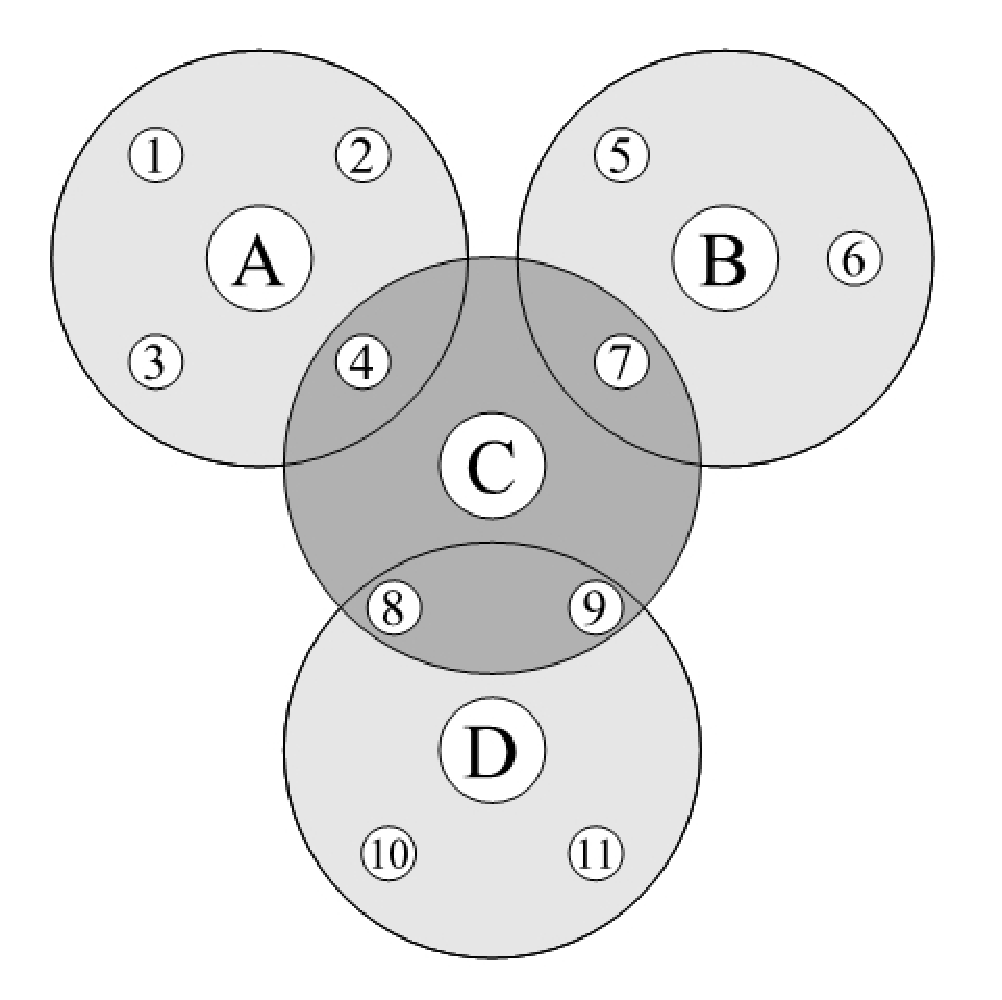
\includegraphics[width=0.4\textwidth]{figures/RBS_multihop.pdf}
\end{center}
\caption{RBS Multi-Hop Network Layout. From~\cite{synchronization:RBS}.}
\label{fig:RBS_multihop}
\end{figure}

Another time synchronization protocol introduced in~\cite{synchronization:TPSN} is the Timing-sync Protocol for Sensor Networks (TPSN). In contrast to RBS, TPSN synchronizes a set of notes to a single global time source. A hierarchical structure is established before synchronization can take place. Once the structure is in place, the root node begins to synchronize all nodes directly connected to it. Those nodes then do the same for their children nodes, etc...

TPSN utilizes the sender-receiver approach~\cite{synchronization:NTP} to synchronize a pair of nodes. A two-way message exchange provides enough information to calculate the clock difference and propagation delay between a pair of nodes. In order to synchronize the whole network, the root node initiates the process. In order to reduce packet collisions, each child node waits for a random amount of time before synchronizing to the parent. This is then repeated with the next level of nodes until they are all synchronized. Due to the very structured nature of TPSN, special protocols are provided for dealing with dying nodes, as well as newly introduced ones.

One of the costs of using TPSN over RBS is that the \emph{Send Time} is once again a source of error in the system. This is, however, mitigated by closely integrating TPSN at the Medium Access Control (MAC) layer. TPSN requires that both incoming and outgoing messages be timestamped at the MAC level in order to minimize uncertainties in transmit and receive times. 

The Flooding-Time Synchronization Protocol (FTSP)~\cite{synchronization:FTSP} is another protocol specifically designed for resource limited wireless platforms. Like TPSN, FTSP relies on MAC-layer time-stamping, along with several other new techniques, to synchronize devices. FTSP uses a single message to synchronize the clocks of to wireless nodes. By comparison, RBS uses a single message to synchronize the clocks of several devices to one-another, but not to the senders clock. TPSN uses two messages to synchronize two device clocks. Because of this, FTSP needs to account to other sources of error, such as the \emph{Byte Alignment Time}. All three protocols are susceptible to the jitter in \emph{Interrupt Handling Time}.

In FTSP, each device sends a broadcast message with its clock time. Devices in the vicinity listen to the broadcast and calculate the difference between their local and received times. In order to reduce jitter, FTSP records multiple times to compute a singe, more accurate time-stamp. This occurs on both the sending and receiving sides. 

Another important contribution from FTSP is a method to deal with clock drift. Due to differences in the exact frequency between local clocks, the time-difference between them grows over time.~\cite{synchronization:FTSP} proposes a solution that takes place off-line. In the short-term, the clock drift is fairly linear. Because of the linear fashion of clock drift, linear regression can be used to distribute the error over a period of time. If clocks are being synchronized every \emph{X} seconds, and clocks drift some amount \emph{Y}, the algorithm distributes the drift \emph{Y} over all samples in a \emph{X} second interval. The reason this must be done off-line is because \emph{Y} can only be computed after each synchronization. 

FTSP scales well to multi-hop wireless networks. Reference points are utilized to keep track of the time differences between the root node and the local node. FTSP is also resistant against losing nodes as it includes root  re-election protocols in case the root node fails. According to ~\cite{synchronization:VHT}, FTSP is currently the \emph{de facto} time synchronization protocol in wireless sensor networks.

The Gradient Time Synchronization Protocol (GTSP)~\cite{synchronization:GTSP} focuses on synchronization of close-by nodes in multi-hop networks. If two physically nearby nodes are part of two different synchronization trees, their clocks might be different. GTSP uses radio broadcasts overheard from all neighbors in order to provide a more accurate time in relation to close-by nodes.

There are certain disadvantages to each of these methods. RBS requires additional messages for time synchronization across multi-hop networks. TPSN does not account for the clock drift of sensor nodes. Both RBS and TPSN are vulnerable to jitter in interrupt handling and decoding times. While FTSP accounts for interrupt handling jitter, it does not take propagation time into account. This is not a problem if nodes are physically close, but can affect performance in long distance cases. GTSP and RBS are also vulnerable to propagation delay errors.

\subsection{Synchronized Sampling}
There are several applications, such as monitoring an active volcano ~\cite{applications:volcano}, structural monitoring~\cite{applications:structural} and counter sniper systems~\cite{applications:sniper}, which rely on synchronized measurements across sensor networks. Currently there is not much research focusing specifically on synchronized sampling in low-power WSNs. Apart from ~\cite{sampling:earthquake}, most research utilizes the previously described time synchronization protocols to keep device clocks aligned. With synchronized clocks, synchronized sampling is no longer a complex problem.

\subsection{Routing and Relaying}
Due to power and physical constraints, sensor nodes placed along the body may not be able to communicate with the main node directly. Even when sensor nodes are able reach the main node, the power required to do so could be prohibitive. The use of relays to re-transmit the data has been shown to dramatically reduce power consumption in body sensor networks~\cite{relay:creepingwave}.

There are several routing protocols currently used in WSNs~\cite{survey:wirelessrouting}, unfortunately, most are not well suited for BSNs. Several of the protocols focus on mobility, Quality of Service (QoS), scalability and reliability, among other things. In general, BSNs do not have the same requirements as other WSNs. For example, in BSNs, scalability is no longer a problem since networks are limited to a human body. In most cases, power consumption becomes the main limiting factor for overall system performance. 

Some routing protocols are specifically designed with BSN constraints in mind. One example is the Wireless Autonomous Spanning tree Protocol (WASP) \cite{protocol:WASP}. Braem et al. describe the WASP as ``a slotted protocol that uses a spanning tree for medium access coordination and traffic routing''. The main idea is that each node sends a ``WASP-scheme'' through a broadcast message that both parent and children nodes receive. This scheme contains the time allotments for each node for the current time frame. The children of the current node need the scheme to know when they are allowed to transmit data. The scheme also informs the parent of the current node as to how many children each node has, which allows it to allocate enough time slots for that branch. This method allows for a distributed time-allocation protocol. Each time frame also includes contention periods where new nodes can join the network. Routing is simple as data from sensor nodes is just sent up the network tree and broadcast messages are used to send configuration down from the root node. The main disadvantage of the WASP is the need to send the scheme packets from the root node down the tree during every time frame.

An improvement over the WASP is the Cascading Information retrieval by Controlling Access with Distributed slot Assignment (CICADA) protocol~\cite{protocol:CICADA}. The improvement over the WASP has to do with the separation of control and data subcycles. The WASP re-configures the time slots during every frame, which produces a significant time delay. The information has to move from the root node to all the children and back. The CICADA protocol configures the network in a separate subcycle and later transfers data. The data transfer is initiated from the bottom of the tree, so there is no delay waiting for the root node to send configurations down during each data subcycle.

Other BSN routing methods focus on postural mobility~\cite{routing:storeandforward}. Quwaider et al. propose a protocol tolerant to constant network changes due to body/sensor movement. When sensor nodes are located in body extremities, the wireless links vary with body position changes. The proposed protocol uses a store-and-forward method to transfer data from sensor nodes to the main node. While the protocol is well suited for dealing with mobile nodes, it requires more energy to do so. ``Hello'' packets are constantly sent by each node to determine what the current neighboring nodes are. A neighbor table is generated using this information and is necessary to determine where packets will be sent to. Another problem with the method is due to multiple copies of packets being transmitted to increase the probability of delivery. Finally, the main node transmits at full power in order to poll each sensor node, increasing its energy consumption.

Most current routing methods for BSNs use network trees. One of the main problems present with network trees is that the nodes closer to the main node deplete their energy supply faster than children nodes. This is due to the fact that all trafic from children nodes has to be relayed through. Ehyaie et al. propose using dedicated relay nodes instead of having sensor nodes act as relays~\cite{relay:networklife}. Using dedicated relays increases the individual sensor life, with the added cost of more devices.

So far, most BSNs have used tree-like networks to join nodes together. Tree networks, while simple, are negatively affected by node failures and movement.  Nabi et al. use a gossiping data routing strategy along with TDMA based MAC to transmit information to the main node \cite{relay:transmitpoweradaptation}. Each node receives and stores the last sample data from every neighboring node. During transmission, it sends its own sampled data, along with one or more of the stored packets from other nodes. This method maximizes the likelihood of a packed reaching the main node, while consuming more power due to retransmissions of the same data. Timestamps are used to decide whether or not a received packed will be stored or discarded. The main node is assumed to have higher battery capacity and transmission range. It is required to be able to reach all nodes with a single transmission. It is in charge of sending a synchronization beacon to use as a time reference for TDMA frames. This method is not always feasible, for example, when two nodes are on opposite sides of the body.

Another valuable contribution from~\cite{relay:transmitpoweradaptation} deals with Transmit Power Adaptation (TPA). The goal for TPA is to minimize power consumption while maintaining a specific link quality. It achieves this goal by adjusting Tx power according to link quality. Unlike the link quality metric in ~\cite{routing:storeandforward}, which was bidirectional, nodes have both inlink and outlink qualities. The outlink metric is then maintained within predefined thresholds by varying Tx power. Inlink quality is stored and later transmitted in order to share the information with neighboring nodes.

\subsection{Similar Work}
In order to determine the improvements of novel methods, reference systems need to be available to compare with. Both~\cite{mac:tdma}~and~\cite{mac:lowdutycycle} provide a suitable reference system for a synchronized, non-relaying BSN. Both proposed systems present, in detail, a TDMA MAC protocol specifically designed with energy efficiency in mind. Details of packet format, TDMA frame calculation, and power consumption measurements are available.
%Add more details later


%[The current system is further simplified by the complete determinism of network traffic. Each sensor node is continuously sampling data at a known rate and sending it back to the main node at known intervals. This allows for protocol simplifications and other energy saving things EXPLAIN!!! ]
 %uncomment to include literature survey


\section{Software Libraries}
One of the primary contributions of this project consists of software libraries for working with WBANs. Due to the project requirements, a choice was made to use free and open source tools, as opposed to proprietary software. Because of this choice, most of the radio libraries had to be either ported or re-written from scratch. There were two main hardware devices that were targeted in these libraries. The first consisted of a CC430 device, which has a built in 915MHz radio. The second was an MSP430 with an external CC2500 2.4GHz radio.

\subsection{Project History}
The first software libraries were initially developed by Corey Provencher, a student at RIT, for a senior design project. He developed a hardware board with a variety of sensors to measure body movements and the corresponding software to use it. All of his software development was done using the Texas Instruments (TI) software tools on Windows(TM).

Jeffery Robble, another student, took over and ported most of the code to use Linux based open source tools. The code ported over by Robble used TI's radio stack \emph{SimpliciTI}. Unfortunately, SimpliciTI was too complex and resource heavy to do time-sensitive operations, like clock synchronization, over the radio. It also required the use of other TI software libraries in order to work.

After Robble left, the work continued. The main goal of the project at the time was to develop wireless electrocardiogram(ECG)(Section~\ref{section:wirelessecg}). While planning for the wireless ECG, a decision was made to develop an entire WBAN platform that could later be used for other projects. The new platform would be developed in-house and included both hardware and software. Because of this, the entire library was to be written from the ground up. This would prevent any rights issues from coming up if published.

\subsection{Design Choices}
The decision to write all software libraries from scratch was not an easy one. Initially the SimpliciTI libraries were modified to try and meet the project needs, but this proved to be a complex task. Due to the simple nature of the planned WBAN, a much less complex approach could be used. The main application only required streaming data from various wireless sensors.$\ll$ Should I elaborate on the design constraints here? The number of devices is known, the time of transmission is known etc...$\gg$ This could be accomplished with a very minimal radio library.

\subsection{CC430 Device}
The first device used in this project was Provencher's initial hardware platform. Due to the limited quantities of that device, a new version of the hardware platform was developed. The new device removed all unused sensors from the board to minimize its footprint. It included a CC430 device with a 32.768Khz crystal oscillator for precise timekeeping. The analog-to-digital(A/D) ports were used to attach any needed sensors. 

Libraries were written for serial communication, visual indicators, analog measurements, time synchronization and radio communications. The serial communication was used to transmit data to the host computer, while the rest were used in the wireless ECG application.

\subsection{MSP430-RF2500 Device}
The second major hardware platform was the MSP430-RF2500. This device is manufactured by TI and sold as a development platform. The MSP430-RF2500 device consists of an MSP430 microcontroller and a CC2500 radio. There were several reasons why this device was used. The primary use for the MSP430-RF2500 was to develop the libraries to use the CC2500 radio. The next planned hardware platform for the project consisted of a CC430 with a CC2500. The previous software libraries would need to be expanded to include a second radio for communication.

Unlike the CC430, which has a radio core built in, the CC2500 is a standalone unit. In order to expedite the software development process, a working platform was needed. Software development new, untested, hardware is not a feasible option. Debugging both hardware and software simultaneously is not a good idea.

The previously developed CC430 libraries were ported to work with the MSP430 microcontroller and expanded to use the CC2500 radio. Features of the new radio libraries include power control, addressing and channel switching.

\section{Specialized Cost Function for Maximizing Body Area Networks Lifetime Using Global Routing Algorithms}
$\ll$ Insert most of the paper here. $\gg$


\section{Wireless ECG Application}\label{section:wirelessecg}
\subsection{Description}
The main goal of the Wireless ECG application is to produce the equivalent output of a traditional, wired, 12-lead ECG using three wireless sensors. 

The three main parts of the wireless ECG project are: 
\begin{itemize}
\item Developing the analog front-end to measure the biopotential signals from the subject.
\item Developing the software/firmware libraries to measure, store, and transmit the data from the EDs to the host.
\item Developing the lead reconstruction algorithms to convert the 3 measurements back to a physician friendly 12-lead display.
\end{itemize}
The work presented here focuses on the software/firmware development for the application.

\subsection{TinyOS Platform}
The first wireless ECG platform was developed using the Imperial College London BSN Motes, which use the TinyOS operating system. These devices are programmed in a derivative of the C language called NesC. While working with these devices and operating system was not particularly simple, the hardware worked, and had been used in other projects. A full 3-sensor wireless ECG application (minus the lead reconstruction) was implemented with these devices. Since the devices run an operating system, several, non-ideal, modifications were required to obtain precise time synchronization.

\subsection{CC430 Platform}
After demonstrating the system using the TinyOS devices, the development of the in-house system continued. After several hardware implementations, a similar 3-sensor wireless ECG application was developed. In contrast to the TinyOS system, the CC430 platform only used hardware and software that was developed by the team.

\subsection{Time Synchronization}
The method used compensates for time offsets between samples and minimizes the effect of clock drift by periodically synchronizing independent clock sources together. Figure~\ref{fig:network_layout} shows an example system consisting of three end devices (\emph{ED}s), one access point (\emph{AP}) and one host computer. 
\begin{figure}[htb]
\begin{center}
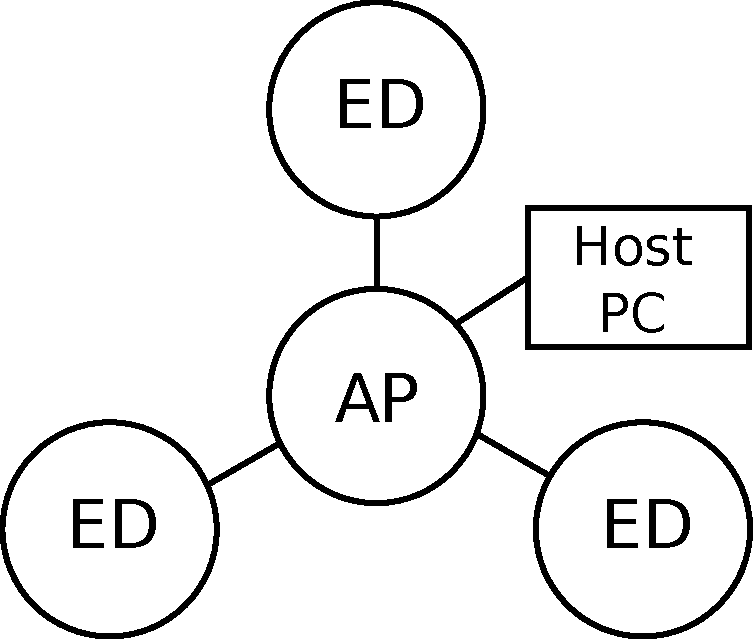
\includegraphics[width=0.4\textwidth]{figures/network-map-test2.pdf}
\end{center}
\caption{Test Network Layout}
\label{fig:network_layout}
\end{figure}
All devices have a timer used for time-stamping and synchronization. All events, including samples and data transfers, occur according to the value of the timer. Due to certain hardware limitations, the value of the timer cannot be altered, it can only be reset to zero. This does not, in any way, affect the synchronization of devices.

The timer inside the \emph{AP} can be considered the primary, or global, timer. The goal is to synchronize all \emph{ED}, or local, timers with the global timer. Whenever the global timer reaches its maximum value, and rolls over back to zero, the \emph{AP} sends a broadcast synchronization beacon instructing each end device it is time zero. When an \emph{ED} receives this message, it compares its current timer value to zero, to calculate the clock drift, and resets it to zero. This ensures that all \emph{ED} timers are aligned, which then allows measurements to occur at close to the same time.

While many, more precise, time synchronization methods are available~\cite{synchronization:FTSP}, it was determined that they were not needed. Due to the low sampling rate and the use of crystal oscillators to run the timers, the precision obtained with this simple method was good enough for the system. More complex methods would not have significantly improved results. Figure~\ref{fig:sync_data} shows the result of three separate wireless devices measuring the same signal. This method was used to confirm that the samples were aligned.

\begin{figure}[htb]
\begin{center}
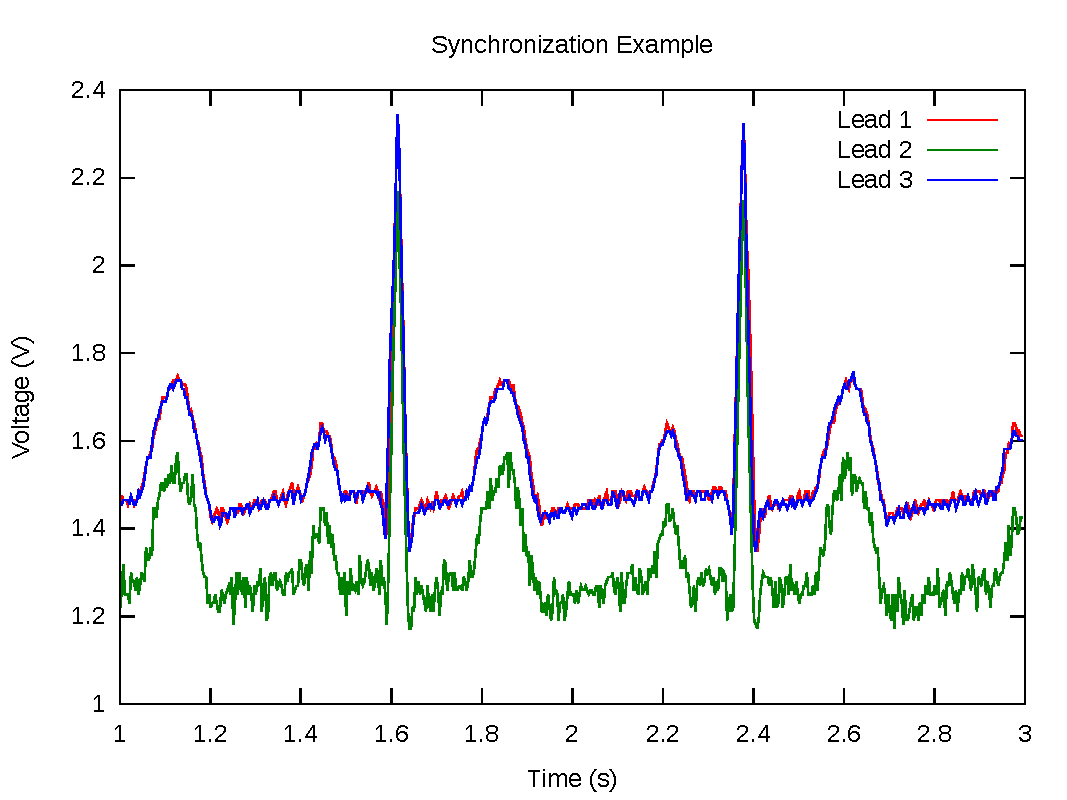
\includegraphics[width=0.8\textwidth]{figures/syncdata.pdf}
\end{center}
\caption{Synchronization Test}
\label{fig:sync_data}
\end{figure}

\subsection{Scheduling}
A round robin-like scheme is used to poll devices in the network. It focuses on simplicity and portability.

In previous implementations, each \emph{ED} was polled individually for sampled data, which required all \emph{ED}s to be on at all times. Once all device clocks are synchronized, polling is no longer necessary. Instead of sending poll messages to each device, the \emph{AP} just listens for \emph{ED} transmissions. The \emph{ED}s will wake up when they are scheduled to transmit and send the required data automatically. This method greatly reduces the power consumption of both \emph{AP} and \emph{ED}s. After initialization, the \emph{AP} only needs to send a periodic time synchronization beacon and the collected data back to the host computer. Once synchronized, end devices will only need to turn their receiver on around the time the synchronization beacon is expected.

Figure~\ref{fig:system_schedule} shows a sample system schedule. The figure shows the time each device is on, and the state of each radio. The ``sleep'' time for each \emph{ED} does not show when a device wakes up to sample data. In this specific case, the \emph{AP} has one extra time-slot allotted for a fourth \emph{ED}.

\begin{figure}[htb]
\begin{center}
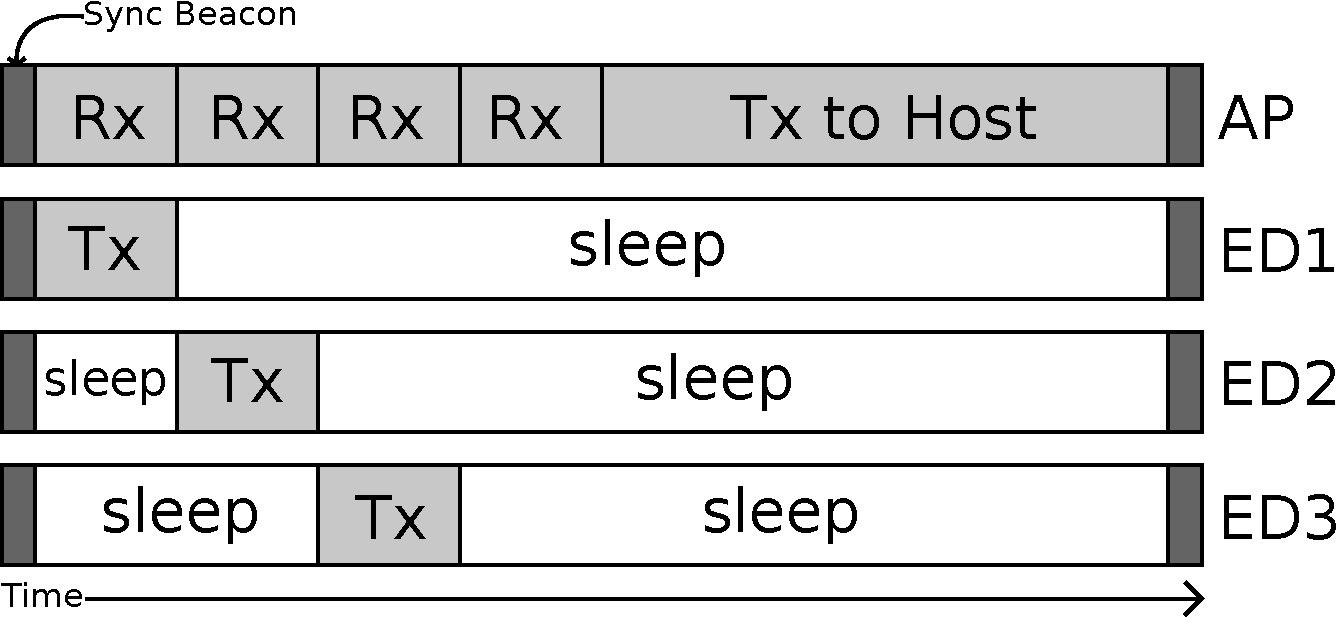
\includegraphics[width=1\textwidth]{figures/sync_schedule.pdf}
\end{center}
\caption{System Schedule}
\label{fig:system_schedule}
\end{figure}

Certain devices can further reduce power consumption by sampling without using the main processor. This works by using direct-memory access(\emph{DMA}) which allows the analog-to-digital converter(\emph{ADC}) to store measurements in memory without first going through the processor. Using this method, Figure~\ref{fig:system_schedule} accurately presents the time each \emph{ED} is powered on. Sampling with DMA has not been implemented in the current wireless ECG platform.

\subsection{Host Interface}
The primary focus of this project was to obtain synchronized samples from several wireless devices. A secondary, but important, goal was to display the data in real time. To speed up development, the live-plotting tool kst(http://kst-plot.kde.org/) was used. A application, written in C, communicated via a USB-to-Serial link with the AP and received all of the ED data. It then output the data to CSV files, which were then used as an input for kst. Figure~\ref{fig:heartbeats} shows an ECG lead wirelessly measured from a human subject.

\begin{figure}[htb]
\begin{center}
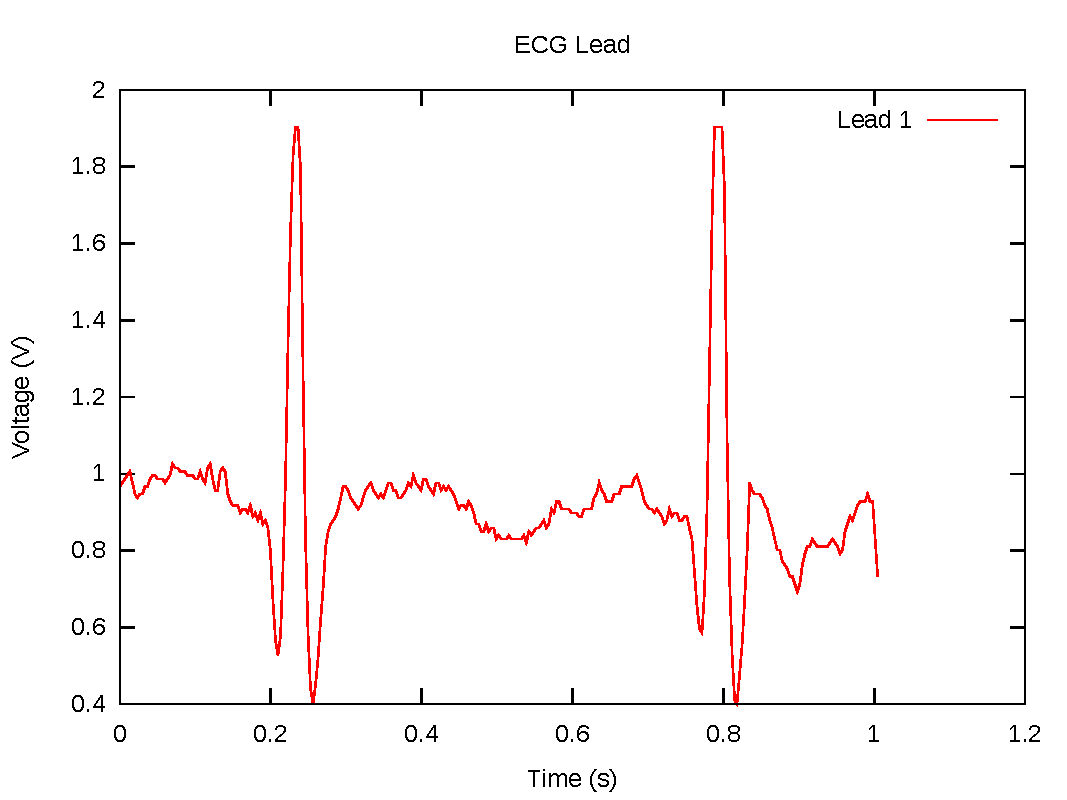
\includegraphics[width=1\textwidth]{figures/heartbeats.pdf}
\end{center}
\caption{Sample Measurement from Single ECG Lead}
\label{fig:heartbeats}
\end{figure}

\section{Conclusion}
...

\pagebreak

\listoffigures

%\listoftables

\bibliography{sources/thesis.bib}{}
\bibliographystyle{plain}
\end{document}